\chapter{Real time Emergency Response(rtER) }
\label{chap:figtab}

\section{Introduction}

I will describe my work related to our Real Time Emergency Response (rtER) prototype system.As described by Smith et al. 
\begin{munquote}[~\cite{rter2013}]
"It is designed to help manage real-time information during a crisis, largely focused on identifying and filtering the most critical information. The real-time Emergency Response project deals with the detection, observation, and assessment of situations requiring intervention by emergency responders. It offers them access to high-quality live data that may be visualized effectively both by responders in-situ and by remote operators in dedicated control rooms.
Unlike other systems that focus on still images and textual content, rtER also incorporates live video feeds.
\end{munquote}
 It also explores the utility of establishing a two way link between a person shooting a video from a smartphone camera and the other person directing the view of the camera from a remote location, to guide them to a better vantage point, implemented seamlessly into the web-based
user interface. The system has following components
\begin{enumerate}
	\item Smartphone application.
	\item Web server component.
	\item Client web application.
	\item An immersive visualization environment.
\end{enumerate}\cite{rter2013}

  
In emergency response and crisis management, the flow of information is tightly controlled through institutionalized hierarchical channels. 
\begin{munquote}[~\cite{rter2013}]
Public perception can be key in preventing mass panic and maintaining public cooperation. The users of the different strata of group activity are:
\begin{itemize}
\item First Responders or Emergency Response Team (ERT): need filtered information or results as immediate action needs to be taken
\item Bystanders: provide real-time information and reports, may be unreliable 
\item Public Information Officer (PIO), typically situated at the emergency operations center (EOC), where coordination and dispatch are handled   
\item Virtual volunteers, arranged in different “trust” levels, and work closely with the PIO
\item The general public
\end{itemize}
\end{munquote}
The use of the different technologies developed, serve different user groups as illustrated in Figure~\ref{fig:infotiers}
\begin{figure}
\begin{center}
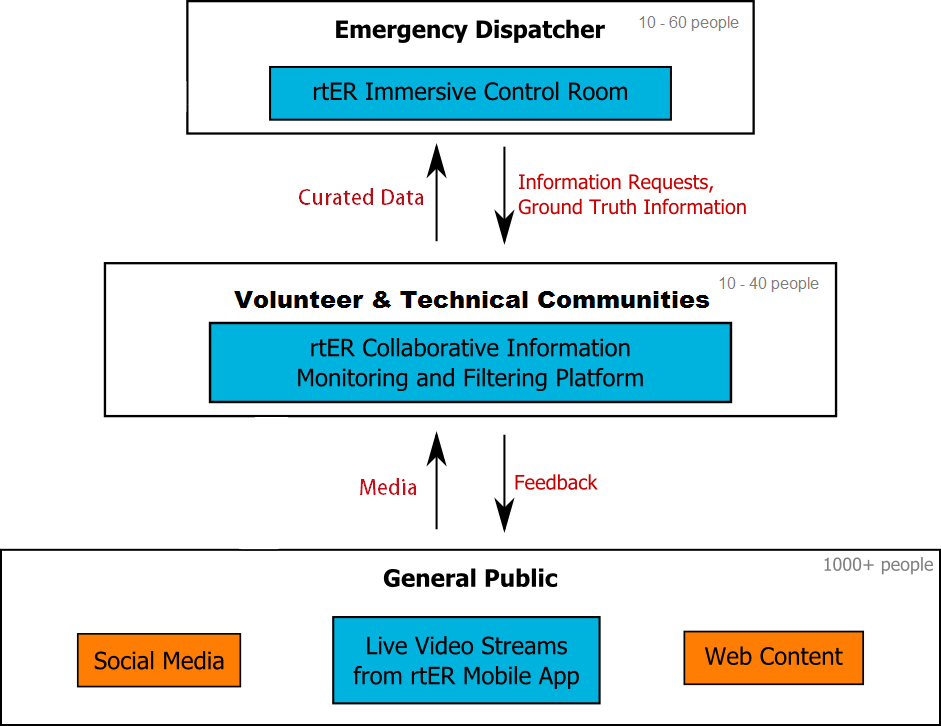
\includegraphics[scale=0.2]{InformationTiers.png}
\caption{Information tiers in the Real-Time Emergency response concept.}
\label{fig:infotiers}
\end{center}
\end{figure}
\section{Problem}
The following scenario (based on real-life events) helps understand the motivation for building rtER.

\begin{munquote}[~\cite{rter2013}]
A 48-inch water main broke at the top of the hill that descends into downtown Montreal, right through the main McGill campus. There was massive flooding through all of the streets and into many of the buildings on the surrounding campus, with black ice underneath, making it practically impassable in many spots. The campus was almost completely surrounded by water making it challenging to find a way off campus.

Jeff left just after the main break, but before any official news had been sent. He could not get off campus easily since the water was flowing too deep and fast through the streets, and had no way of figuring out how far the situation spread without slogging through knee-deep water. There were many students and others standing around with cameras taking pictures and video all around campus (later dozens of videos were posted online) and posting on social media.

For those in the buildings trying to plan their way home, being able to see these images, videos and tweets might have been helpful. But without some way of sorting and filtering it might also simply have been overwhelming.

We imagine that rtER would have helped us solve this problem. By allowing information---video, image or text---to be visualised in geographic context on the rtER map, users could have quickly understood what was occurring where. Moreover, filtering using the map would have provided a way for those looking for a way of campus to eliminate all superfluous information and see only the information coming from one area on their map. This would mean you could quickly confirm or deny if a route was safe.

Since we are trying to build our system with collaboration in mind, repetitious search would be avoided and time could be saved. For example in this case most people posting pictures and videos were ``ambulance chasing'' by showing the drama and devastation, not the less interesting safe area. This means that the ``useful'' information was being buried by the ``shock value'' videos. Once a person had found a safe passage using our system, via a tweet suggesting a safe route or possibly a picture or a video showing an unflooded area, they could promote that information to higher priority for others to see. As a result the next person wouldn't need to repeat that search. They might instead simply add a confirmation after using the route, or perhaps provide an alternative. In this way we hope our system may make a more efficient use of human resources.”
\end{munquote}



\section{System Architecture}
I have been involved in the development of two components of the whole system, viz., the android client application and the client web application.



\subsection{Collaborative information web client}
The web client was developed for the virtual operations support teams\munfootnote{http://idisaster.wordpress.com/2012/02/13/what-is-a-virtual-operations-support-team/}(VOSTs). With the increasing public participation in emergency response, the number of incoming videos and social media streams can easily overwhelm the EOC personnel. The tool developed for this group of users, built around a web client (Figure~\ref{fig:clientscreen}), can be used by emergency responders to curate information including live video, Twitter feeds, YouTube and other social media.  My worked was focused on Twitter integration in the Web Client.
\begin{figure}
\begin{center}
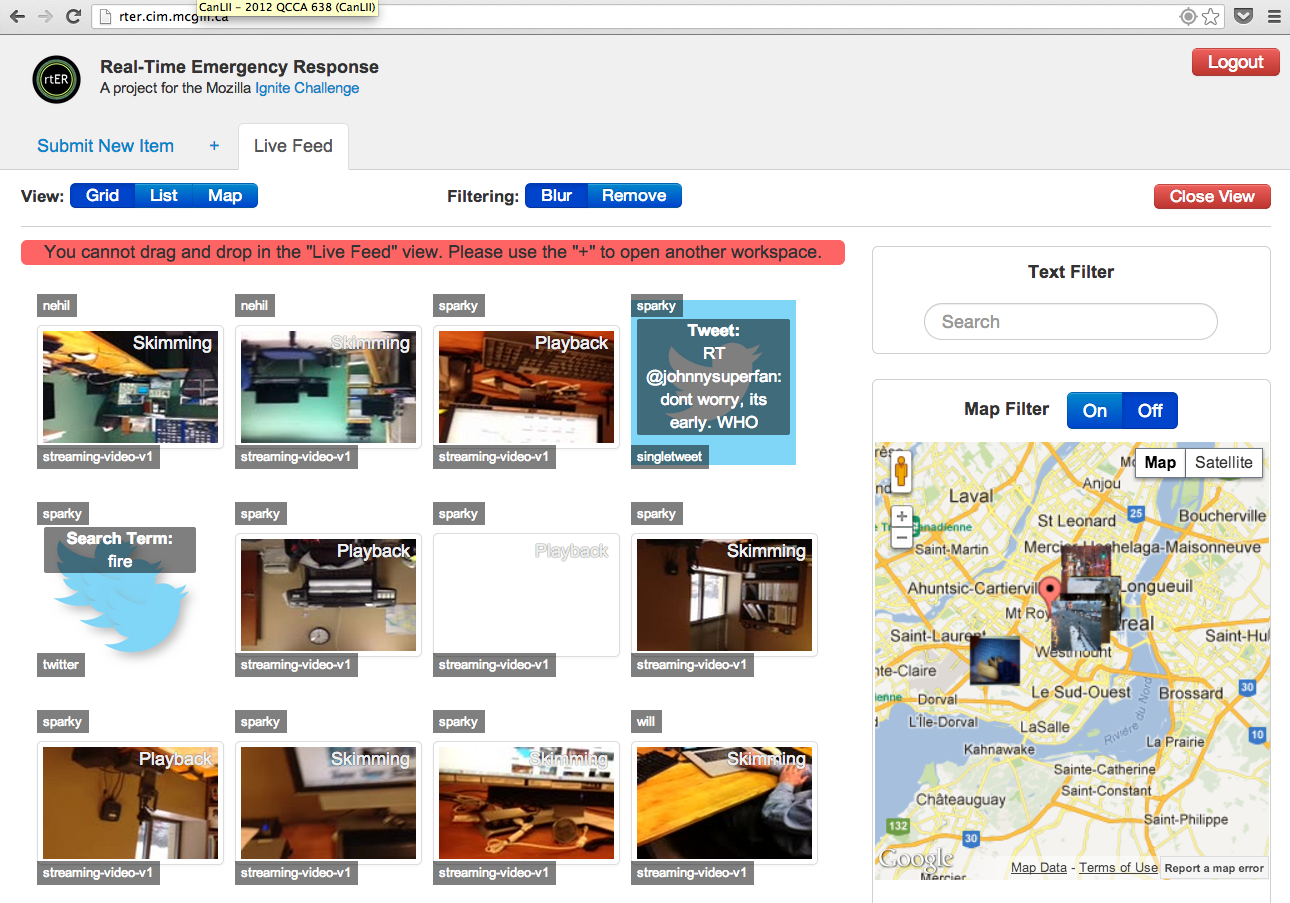
\includegraphics[scale=0.3]{clientscreen.png}
\caption{The Web Client UI, displaying the video streams and twitter feeds, alongside a map.}
\label{fig:clientscreen}
\end{center}
\end{figure}
\subsubsection{Importance of Twitter in crisis management}
The different stages of any disaster are: 

\begin{enumerate}
\item Warning
\item Threat
\item Impact
\item Inventory
\item Rescue
\item Remedy
\item Recovery
\end{enumerate}
Micro-blogging has been proven to be highly effective as one of the useful tools in stages 3 to 5 according to the above taxonomy. During these stages, more traditional communication channels are less effective than the emerging ICT ones. Twitter tends to describe a common/global topic, diminishing the network entropy. This makes Twitter an indispensable tool \cite{Mendoza:2010:TUC:1964858.1964869}.

The backbone of the web client is HTML5 and AngularJS\munfootnote{Angular JS - http://angularjs.org/}. AngularJS is an open-source JavaScript framework, maintained by Google. The framework adapts and extends traditional HTML to better serve dynamic content through two-way data-binding that allows for the automatic synchronization of models and views. This make our web client app responsive and provides near real-time updates in a particular web view. 

The UI is built using AngularUI\munfootnote{ http://angular-ui.github.io/} and Twitter Bootstrap UI\munfootnote{ http://twitter.github.io/bootstrap/}. AngularUI is the companion suite(s) to the AngularJS framework. It comprises of several components: UI-Module, UI-Bootstrap, NG-Grid, UI-Router and IDE plug-ins. The Twitter Bootstrap UI is a front-end framework for faster and more elegant web development. This framework comprises of responsive css. This makes our web client app have a uniform UI on latest desktop, tablets and smartphone browsers as well.

The present implementation of the web client has two kinds of Twitter Items. 
\begin{itemize}
	\item Twitter search : This is a stream of relevant tweets that match a specified query. This feature uses the Twitter Search API. Get Search API v1 resource url : \texttt{http://search.twitter.com/search.format}. There are three views associated with each Twitter search item in the system, viz., Creation, Close-Up View  and Tile View.
	\begin{itemize}
		\item Create View: The form to create a search query is shown below. The user can build their specific query using 3 options.
		\begin{itemize}
		\item Search Term: The default functionality is to search the term entered in the field as a keyword in the tweet. More complex queries can be constructed using operators. Example Query:\texttt{ "This exact phrase" any OR of OR these OR words -none -of -these -words \#these OR \#hashtags lang:en from:from OR from:these OR from:accounts to:to OR to:these OR to:accounts \@mentioning OR \@these OR \@accounts near:"location" within:15mi :(.} Operators explained
		\begin{itemize}
		\item Words within \texttt{" "} -   This exact phrase
		\item Words separated by \texttt{OR} - Any of these words
		\item Words preceded by \texttt{-} - None of these words
		\item \texttt{lang:} - language selection
		\item Words separated by \texttt{ from: } - from these user accounts 
		\item Words separated by \texttt{to:} - to these user accounts 
		\item Words separated by \texttt{ \@} - mention of these user accounts 
		\item \texttt{near:} - location selection 
		\item \texttt{ :),:( , ? } - Positive sentiment, Negative sentiment, Question, respectively.		
		\end{itemize}
\begin{figure}
\begin{center}
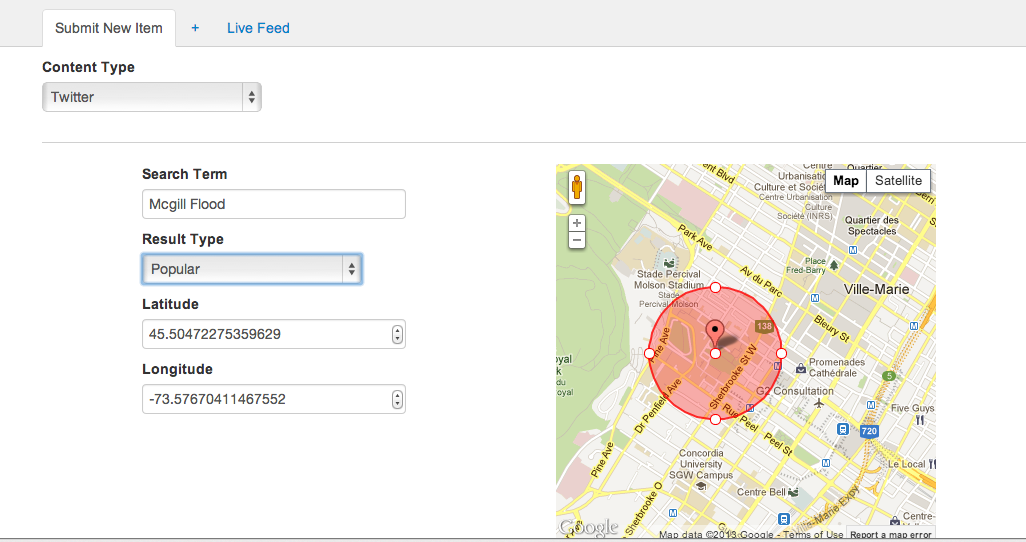
\includegraphics[scale=0.3]{createtwitter.png}
\caption{The image shows the form, used to create a twitter search item, the map shows a circle bounding the McGill University area}
\label{fig:createtwitter}
\end{center}
\end{figure}	
		\item The user can also select the result type of the stream from the following options: 
		\begin{itemize}
		\item \texttt{mixed} - Include both popular and real time results in the response.
		\item \texttt{recent} (Default) - Return only the most recent results in the response.
		\item \texttt{popular} - Return only the most popular results in the response.
		
		\end{itemize}
		\item The user can make the search query location specific also. Using the map view, the user can draw a circular region on the map to define the area of search.
	\end{itemize}
		\item Close Up View : This view displays the stream of tweets resulting from the query. Each tweet can be ‘promoted’ to the common live feed as a ‘single tweet’. Also, the user can ‘react’ to the tweet instantly.
\begin{figure}
\begin{center}
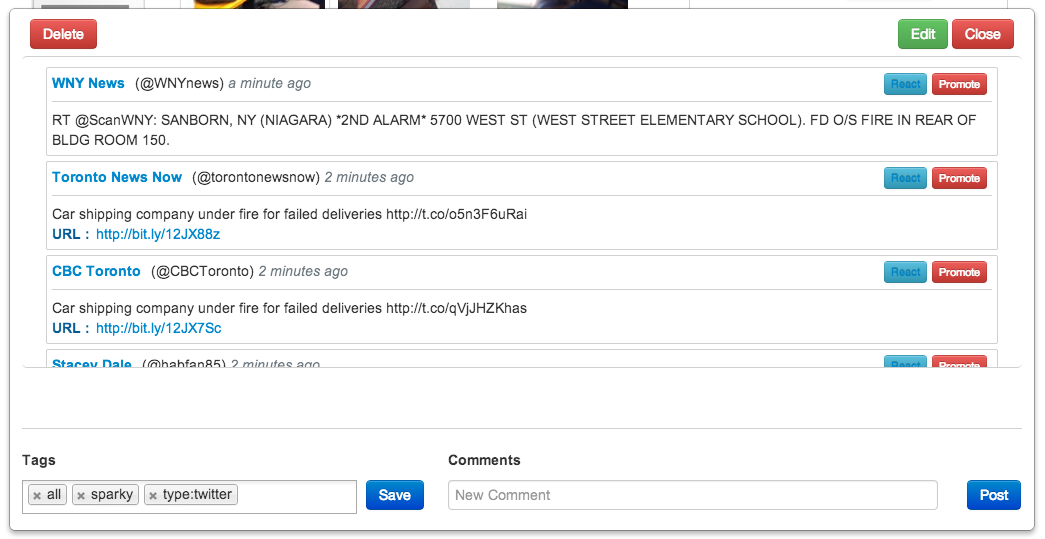
\includegraphics[scale=0.3]{closeuptwittersearch.png}
\caption{The twitter stream of recent tweets on 'fire'}
\label{fig:closeuptwitter}
\end{center}
\end{figure}	
		\item Tile View: This view represents the twitter search item as a part of the live feed in the form of an item of a grid of tiles. This emphasizes on the search term.
	\end{itemize}	
	\item Single Tweet: It is a single tweet that is promoted by the VOST members to promote it into the collaborative workspace.
		\begin{itemize}
			\item Create View: The Single tweet can be created by promoting a tweet from twitter search stream to the mainstream.
			\item Close up Item: The Close-up view displays the tweet card of the particular tweet. A tweet card displays a tweet with expanded media like photos, videos, and article summaries, and also includes real-time retweet and favourite counts. They are interactive and enable the users to follow the Tweet author, and reply, re-tweet, favourite all directly from the page. To achieve this, I used the  oEmbed endpoint of Twitter. Resource url: \texttt{https://api.twitter.com/1/statuses/oembed.format}
\begin{figure}
\begin{center}
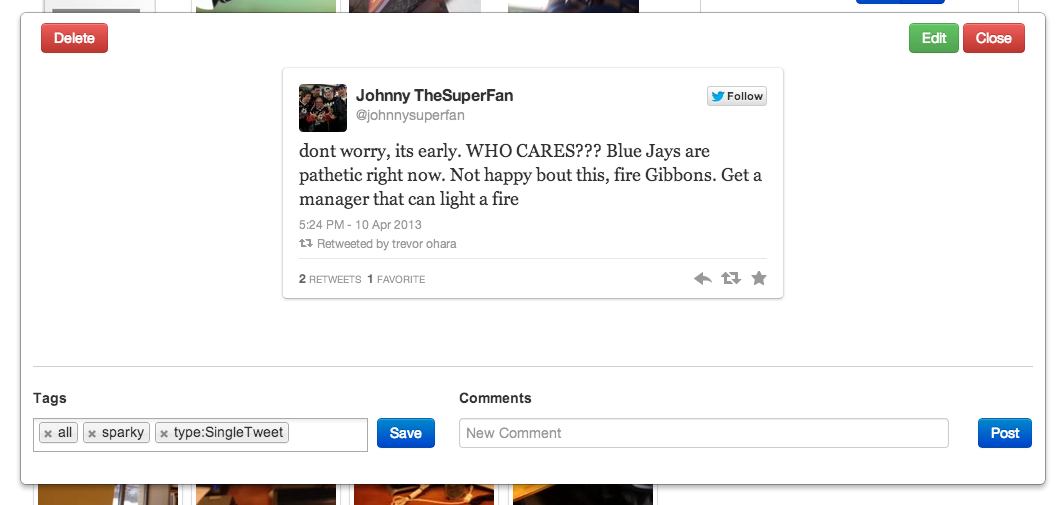
\includegraphics[scale=0.3]{singletweet.png}
\caption{A Tweet Card}
\label{fig:singletweet}
\end{center}
\end{figure}				

			\item Tile Item: This view represents the twitter search item as a part of the live feed in the form of an item of a grid of tiles. This displays the text of the tweet in the tile to get a quick reference to the Single tweet.
		\end{itemize}
	
\end{itemize}

\section{Video Streaming}
As described by Smith et al. 
\begin{munquote}[~\cite{rter2013}]
Previously, our system architecture lacked a robust video streaming architecture.
Our latest video streaming architecture, shown in Figure 7, provides end-to-end scalable and relatively low-latency video from a smartphone source to HTML5 web clients, supporting ingest of multiple simultaneous streams at a server and scalable distribution to multiple simultaneous viewers. We achieve these goals by employing live encoding at the smartphone, transcoding streams into segmented video at a server and delivering video segments to web browsers using HTTP Live Streaming (HLS) [10] in two different formats, MPEG2-TS/H.264 and WebM/VP8. On the ingest side, our smartphone application encodes captured video frames into H.264/AVC [11], encapsulates them into a timestamped MPEG2 Transport Stream and forwards the video frame-wise via HTTP to our streaming server \cite{rter2013}.
\end{munquote}
I have been involved in developing the android client application.

\section{Android Client App}
The typical use case for the mobile app places someone with a smartphone on site in a disaster scenario, ideally situated to provide relevant contextual data to emergency responders, possibly filtered by virtual volunteers. Using the rtER mobile app, the smartphone user streams a video feed, deemed to be relevant, which immediately appears as a live tile to VOST volunteers connected to the rtER web client, where it can be sorted based on its situational importance.

	\begin{itemize}
		\item Version 1 -  For the live video streaming, we used the open source ipcamera{reference required}, a project for android, along with \texttt{Google LibJingle} and \texttt{Nanohttpd}. These provide a peer to peer data transfer from the android device, acting as a server on a wifi network. Timestamped latitude and longitude information obtained using location-based services, are delivered to the server, in parallel to the live stream as a JSON object. This implementation creates a server on the android client which is blocked by the network provider’s firewall. Thus, the live video data cannot be sent.
		\item Version 2 - In this version, we developed a new app from the ground up. It streams jpeg images from the camera and provides a feature for directing the viewer to look at a desired vantage point. This created a two way link between the curator and the user of the app capturing the stream. The images are captured using Camera Class in Android SDK and the desired orientation of the device is indicated by the bounding box created in OpenGL, overlaid on the preview surface of the camera. This is illustrated in the figures below. The frame rate is low because each frame is captured after the previous has been written to the SD card (external storage) of the device. Then it is added into the queue, to be posted to the server.
\begin{figure}
\begin{center}
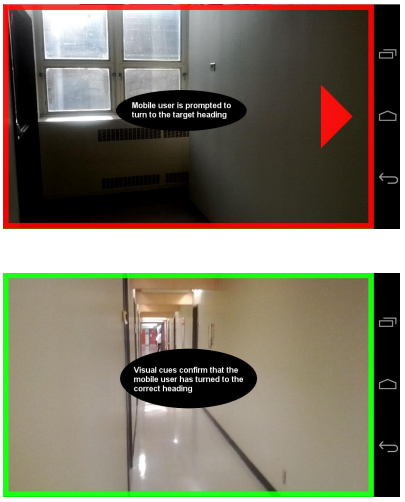
\includegraphics[scale=0.6]{androidv2.png}
\caption{Android App showing two orientation. The Red bounding box indicates that the user should steer to the left and then the colour of the bounding box changes to green as shown below.}
\label{fig:androidv2}
\end{center}
\end{figure}		
		\item Version 3 -Currently, I am working on improving the frame rate to make the stream almost real-time video over 3g network. There are two possible ways to achieve this on android platform:
		\begin{itemize}
			\item \texttt{MediaRecorder} class: This is a class in android SDK, used to record audio and video from the device. The recording control is based on a simple state machine. H.264 encoded video is written to a Mpeg2 TS file. Android SDK Media API is one of the weak points of this platform. The API restricts the developer from writing the recorded data from the camera to a stream. Presently, this data can only be written to a file in the external/internal filesystem of the device. To circumvent this, I plan to write the file to a local socket using java.net.Socket. Network sockets also have file descriptors and they can be accessed using, \texttt{ParcelFileDescriptor}. Using this, we can plug in the video stream data into the socket. On the other end of the socket, we can retrieve the data and use HTTP Post to sent to the video server using \texttt{ChunkedOutputStream} in android. The advantage of this method is, it uses the device’s hardware encoders. This will be faster and computationally inexpensive. We can achieve 30fps stream without any compromises in the performance of the app.
			\item FFMpeg and Libx264: This method involves extracting raw frames from the camera and encoding them to H.264 frames using FFMpeg Library. This can be achieved using Android Native Development Kit (NDK). Then H.264 encoded frames can be individually sent to the server via HTTP Post. The server handles the packaging of these frames into a Mpeg2 TS stream. This method is comparatively slower and less efficient, as it uses more resources on the device. Our iOS implementation  uses the same architecture. The optimum parameters of the video stream transmitted is 15 frames per second (fps) at a resolution of 640 x 360 at 600kbps using iPhone 4s devices. This is susceptible to network congestion.		
		\end{itemize}
	This is a work in progress.	
	\end{itemize}
\section{Accomplishments}
During my project, these were the major accomplishments.
\begin{enumerate}
	\item rtER was Gold prize winning project in Brainstorming round in Mozilla Ignite
	\item Our team is selected to showcase rtER in finale of USA Ignite in Chicago.
\end{enumerate}
